
\section{Introduction}

\subsection{Overview}

\begin{quote}
D3.2) Final field tested Integrated Energy System: Output of T3.1-5; Based on information provided by the deployment of deliverable 3.2 the software is further refined to provide energy services and community management (open source). 
\end{quote}

In the third year of Work Package 3 (WP3), we continued the design and development of the software platform YouPower\footnote{ \url{http://civis.tbm.tudelft.nl/}} based on the results reported in D3.2. In this report, the final results are summarized as a whole for readability and usefulness. The refinement and improvement made in the third year are highlighted when necessary and possible. 
% 
The functionalities of the platform reported are deployed at Stockholm and/or Trento test sites respectively according to the local context. The YouPower software is open source under the Apache v.2 License\footnote{\url{https://github.com/CIVIS-project/YouPower/blob/master/LICENSE}}. It has  an online repository at GitHub\footnote{ \url{https://github.com/CIVIS-project/YouPower/}}. 
The backend API documentation is aslo available online\footnote{ \url{http://civis.tbm.tudelft.nl/apidoc/}}. 


\subsection{Aims and Scope}

As stated in D3.1, past research has typically regarded grid users as individual entities driven by economic considerations, contributing individually to achieve energy goals \citep[e.g.][]{Barbieri2013,Buoro2012,Martinez-Lera2013}. 
A novel research goal of CIVIS is that our research attention is oriented to the potentials and challenges of users' collective action, pro-social values and sense of community. We deem collective human behaviour critical, because it is \textit{both} a source of and a solution to the problem of climate change \citep{Masson2014}.  

To this end, we aim to explore the potential and challenges of supporting social participation, awareness and engagement by means of ICT in the smart grids to achieve sustainable energy goals such as consumption reduction and load shifting. In D3.1, we reasoned that an energy software platform that includes features of Social Network (SN) platforms can be used to form energy prosumer communities. 
% 
On such a \textit{Social Smart Grid Platform} (SSGP), users can share energy-specific interests and values, exchange experiences,  compare energy consumption, and receive actionable information and feedback. 
%
Moreover, we as researchers can use this platform as a communication channel to promote the aforementioned goals. The platform is also a research instrument to observe users' activities (including their self-exposed energy behaviors), responses, and possible outcomes in energy consumption and social impact.  The data collected through the platform will be analyzed in the third year of the CIVIS project.  

\begin{figure}
\begin{center}\footnotesize
	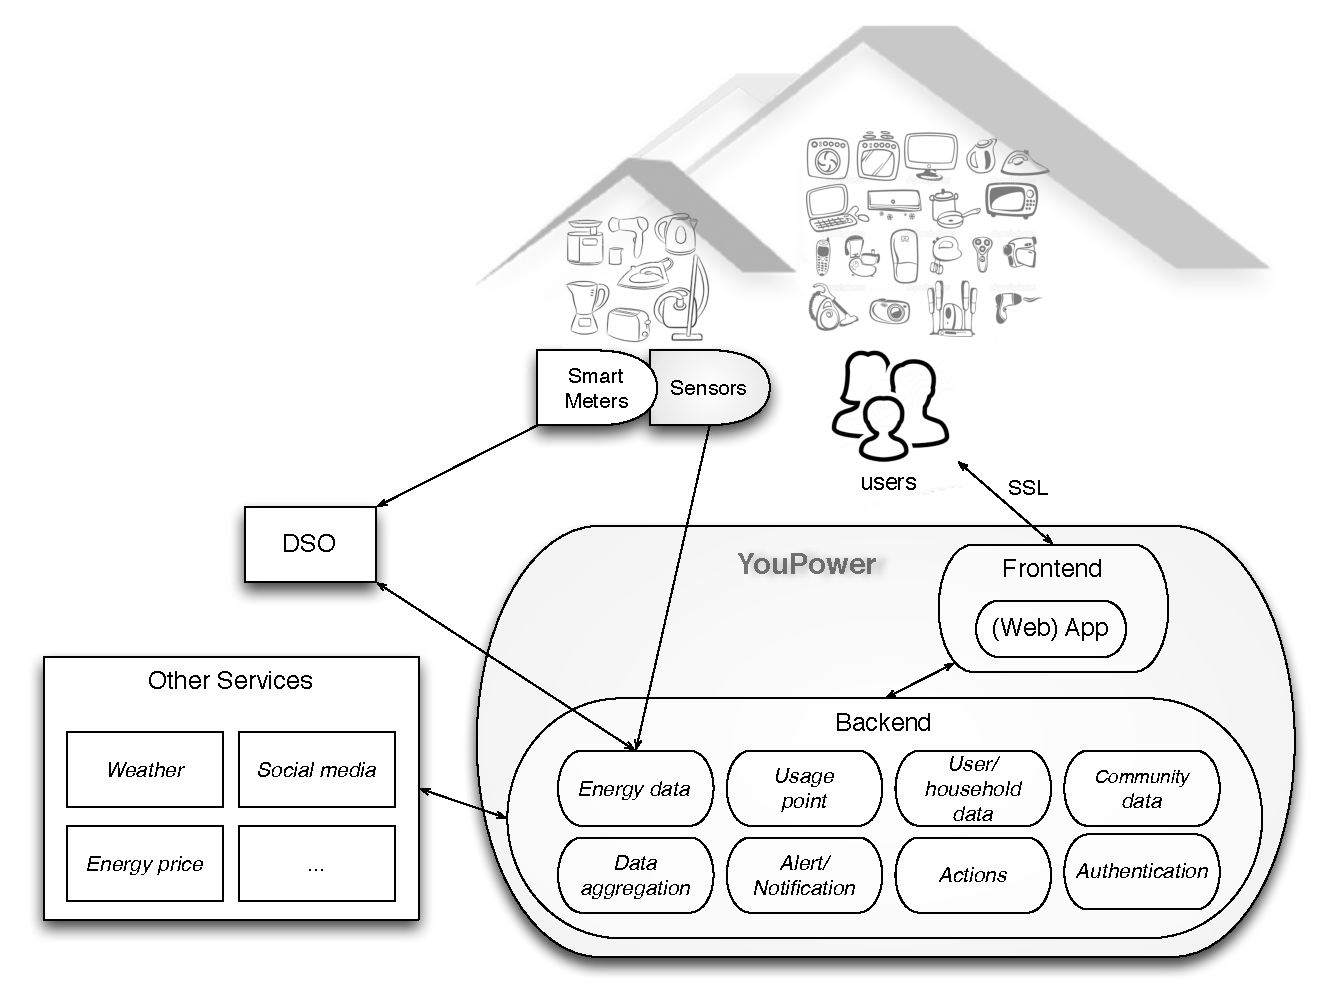
\includegraphics[width=.85\textwidth]{img/civis_platform_overview.pdf}\\
	DSO (Distribution System Operators),  SSL (Secure Sockets Layer)
	\caption{CIVIS platform overview}\label{fig:platform}
\end{center}
\end{figure}
%
Figure~\ref{fig:platform} gives an overview of the CIVIS platform. The scope of WP3 D3.2 is indicated by the dashed circle. The CIVIS platform is composed of services developed by WP3 and WP4 (the CIVIS back-end), and an application (the CIVIS front-end) that interacts directly with users. 
Briefly, WP4 focuses on the system level ICT services that deal with energy data that is collected by smart meters and sensors installed at households in the Swedish and Italian test sites (see D4.2 for more details). 
WP3 focuses on the front-end application and the social level ICT services that deal with user, household and community data. Unless otherwise specified, this report discusses the design and development of the WP3 part of the CIVIS platform which is called \textit{YouPower}\footnote{The CIVIS front-end application used to be called EnergyUP. The old name may be found in some old documents and/or mock-ups.}. The name suggests a non-solipsistic state of mind --- by using ``You'' \citep{Crumlish2009} --- in facing and tackling energy-related issues, with overtones of user empowerment. 

%The authentication of user sign up and login to an EnergyUP account is managed by WP3 services. A user may also choose to link his or her energy data, additional authentication is required. 

%The effectiveness of smart grids depends on consumer engagement and action. Today’s consumers have a vague understanding of the grid. How consumers understand the smart grid will shape how they feel about it, and in turn how readily they adopt it, and how they use it. 
%
%Seeing is believing 
%If consumers are given useful feedback on how they use energy and are provided with recommendations on how to improve, they will have the chances to make more informed energy choices. 
%
%

\subsection{Design and Development Process: the Continuation}

An important research question to be investigated in WP3's second year's activities is: what is a good design of a SSGP that can be potentially successful given the goals and context stated in 1.1 and 1.2. 
% 
We have followed an adaptive agile development process with iterative rapid prototyping \citep{Leffingwell2011}. This is a discovery-based approach where users are actively involved in reviewing and giving feedback to the prototype design from the onset and throughout the process. 

During the period of Oct. -- Nov.~2014, an initial set of CIVIS platform features\footnote{A feature of a system or a product is a high-level expression of a desired system behavior \citep{Leffingwell2000}. } was collected collaboratively using Google Docs. A CIVIS design workshop took place at TU Delft (see D1.2). In several rounds, CIVIS partners proposed candidate features that are potentially useful to the CIVIS plarform based on their knowledge and expertise, informed by user needs and the state-of-the-art.
%

These features were organized into categories and were used as a basis for further discussion in the Telcos during Dec.~2014 -- Jan.~2015 among CIVIS partners. 
As a result, a list of features was selected and prioritized by usefulness, feasibility and practicality. 

In Feb.~2015 we began to make wireframe mock-ups\footnote{A shortened list of YouPower mock-ups can be found at \url{http://civis.tbm.tudelft.nl/mockups/}.} of the CIVIS front-end application. The mock-ups served as visual guides that can be more easily communicated to general users compared to traditional software requirement and design documents. Since then, we continually modified the design (mock-ups) based on the feedback and advices from colleagues, peers and focus group meetings (see D1.2). 

The prototyping was started in May 2015\footnote{The latest version of the prototype can be found at \url{http://civis.tbm.tudelft.nl/frontend.html}.}; the back-end development followed one month later. They evolved into the current version of YouPower, as a proof of concept for a SSGP.  
At the moment of writing this report, YouPower is still in development. It is planned to be deployed at the Stockholm and Trentino test sites by Oct.~2015. 
The CIVIS server at TU Delft hosts the latest deployment of YouPower\footnote{The lastest version (a web-version designed for mobile screens) can be found at \url{http://civis.tbm.tudelft.nl/}. The CIVIS repository at GitHub \url{https://github.com/CIVIS-project/YouPower/} hosts the source code and manages version control.}.

The rest of this report discusses the design and development of YouPower. During the design and development process, we have paid particular attention to quick responses to changes, and adaptive development. In this report, however, limited by time and space, we will skip the intermediate steps and only discuss the end results. 
In Section 2, we first discuss the analytical framework and guidelines we adopted for the CIVIS platform design, and then present the design concept of the CIVIS platform. In Section 3, we give an overview about the technologies and platforms we choose to use for the CIVIS prototype development. The relevant references and resources are added for further information. In Section 4, we review the WP3 tasks and discuss a number of open issues. 

%literature, group feedback (internal), user feedback: workshops, focus groups 
 
